% Copertina per la stampa in brossura: quarta + dorso + prima,
% con 3 mm di abbondanza su tutti i lati. Nessuna linea guida o segno di taglio.
% Larghezza del formato rifilato e spessore del dorso (in mm) si impostano così:
%   xelatex "\def\eoptrimw{165}\def\eopspine{5.5}% Copertina per la stampa in brossura: quarta + dorso + prima,
% con 3 mm di abbondanza su tutti i lati. Nessuna linea guida o segno di taglio.
% Larghezza del formato rifilato e spessore del dorso (in mm) si impostano così:
%   xelatex "\def\eoptrimw{165}\def\eopspine{5.5}% Copertina per la stampa in brossura: quarta + dorso + prima,
% con 3 mm di abbondanza su tutti i lati. Nessuna linea guida o segno di taglio.
% Larghezza del formato rifilato e spessore del dorso (in mm) si impostano così:
%   xelatex "\def\eoptrimw{165}\def\eopspine{5.5}% Copertina per la stampa in brossura: quarta + dorso + prima,
% con 3 mm di abbondanza su tutti i lati. Nessuna linea guida o segno di taglio.
% Larghezza del formato rifilato e spessore del dorso (in mm) si impostano così:
%   xelatex "\def\eoptrimw{165}\def\eopspine{5.5}\input{copertina-stampa}"
% (senza \def: 165 mm di larghezza, 240 mm di altezza, dorso 5,5 mm).
\ifdefined\eoptrimw\else\def\eoptrimw{165}\fi
\ifdefined\eopspine\else\def\eopspine{5.5}\fi
\ifdefined\eopguides\else\def\eopguides{0}\fi
\newdimen\eoppw \eoppw=\dimexpr 2\dimexpr\eoptrimw mm\relax+6mm+\eopspine mm\relax
\documentclass{article}
\usepackage{fontspec}
\defaultfontfeatures{Ligatures=TeX}% apostrofi tipografici ’
\usepackage{tikz}
\usepackage{xcolor}
\usepackage[paperwidth=\the\eoppw,paperheight=246mm,margin=0pt]{geometry}
\pagestyle{empty}
\frenchspacing
\setlength{\parindent}{0pt}
\newfontfamily\eopcoverfont{SourceSans3}[Path=fonts/,Extension=.otf,UprightFont=*-Light,BoldFont=*-Regular,WordSpace={1.9,1.4,1}]
\setsansfont{SourceSans3}[Path=fonts/,Extension=.otf,
  UprightFont=*-Regular,ItalicFont=*-It,BoldFont=*-Semibold,BoldItalicFont=*-SemiboldIt]
\newfontfamily\eopcoverbold{SourceSans3}[Path=fonts/,Extension=.otf,UprightFont=*-Semibold,WordSpace=1.3]
\newfontfamily\eopcoverreg{SourceSans3}[Path=fonts/,Extension=.otf,UprightFont=*-Regular,ItalicFont=*-It]
% testo della copertina: niente sillabazione, righe a bandiera
\newcommand{\eopnohyph}{\hyphenpenalty=10000 \exhyphenpenalty=10000 \raggedright}
% colori in RGB: Ghostscript li converte in CMYK FOGRA51 insieme all'immagine,
% così fondo e foto finiscono con gli stessi valori di inchiostro
\definecolor{eopteal}{HTML}{0097B2}
\definecolor{eopcream}{HTML}{FCE8A2}

\begin{document}
\begin{tikzpicture}[remember picture,overlay,x=1mm,y=1mm]
  % origine: angolo in basso a sinistra del foglio (abbondanza compresa)
  \coordinate (O) at (current page.south west);
  \def\S{\eopspine}
  \pgfmathsetmacro\xs{\eoptrimw+3}               % piega quarta/dorso
  \pgfmathsetmacro\xf{\eoptrimw+3+\eopspine}     % piega dorso/prima
  \pgfmathsetmacro\xc{\xf+\eoptrimw/2}           % centro della prima
  \pgfmathsetmacro\xr{2*\eoptrimw+6+\eopspine}   % bordo destro del foglio
  \pgfmathsetmacro\tw{\eoptrimw-24}              % giustezza del titolo in prima (12 mm dai bordi)
  \pgfmathsetmacro\bw{\eoptrimw-36}              % giustezza dei testi in quarta
  % ---- fondo azzurro: quarta e dorso ----
  \fill[eopteal] (O) rectangle ([xshift=\xf mm+4mm,yshift=246mm]O);
  % ---- prima di copertina: immagine centrata sul rifilo, tagliata ai lati ----
  \begin{scope}
    \clip ([xshift=\xf mm]O) rectangle ([xshift=\xr mm,yshift=246mm]O);
    % immagine allineata alla piega del dorso (il globo resta ad almeno 10 mm), tagliata a destra
    \node[inner sep=0pt,anchor=west] at ([xshift=\xf mm+3mm,yshift=123mm]O)
      {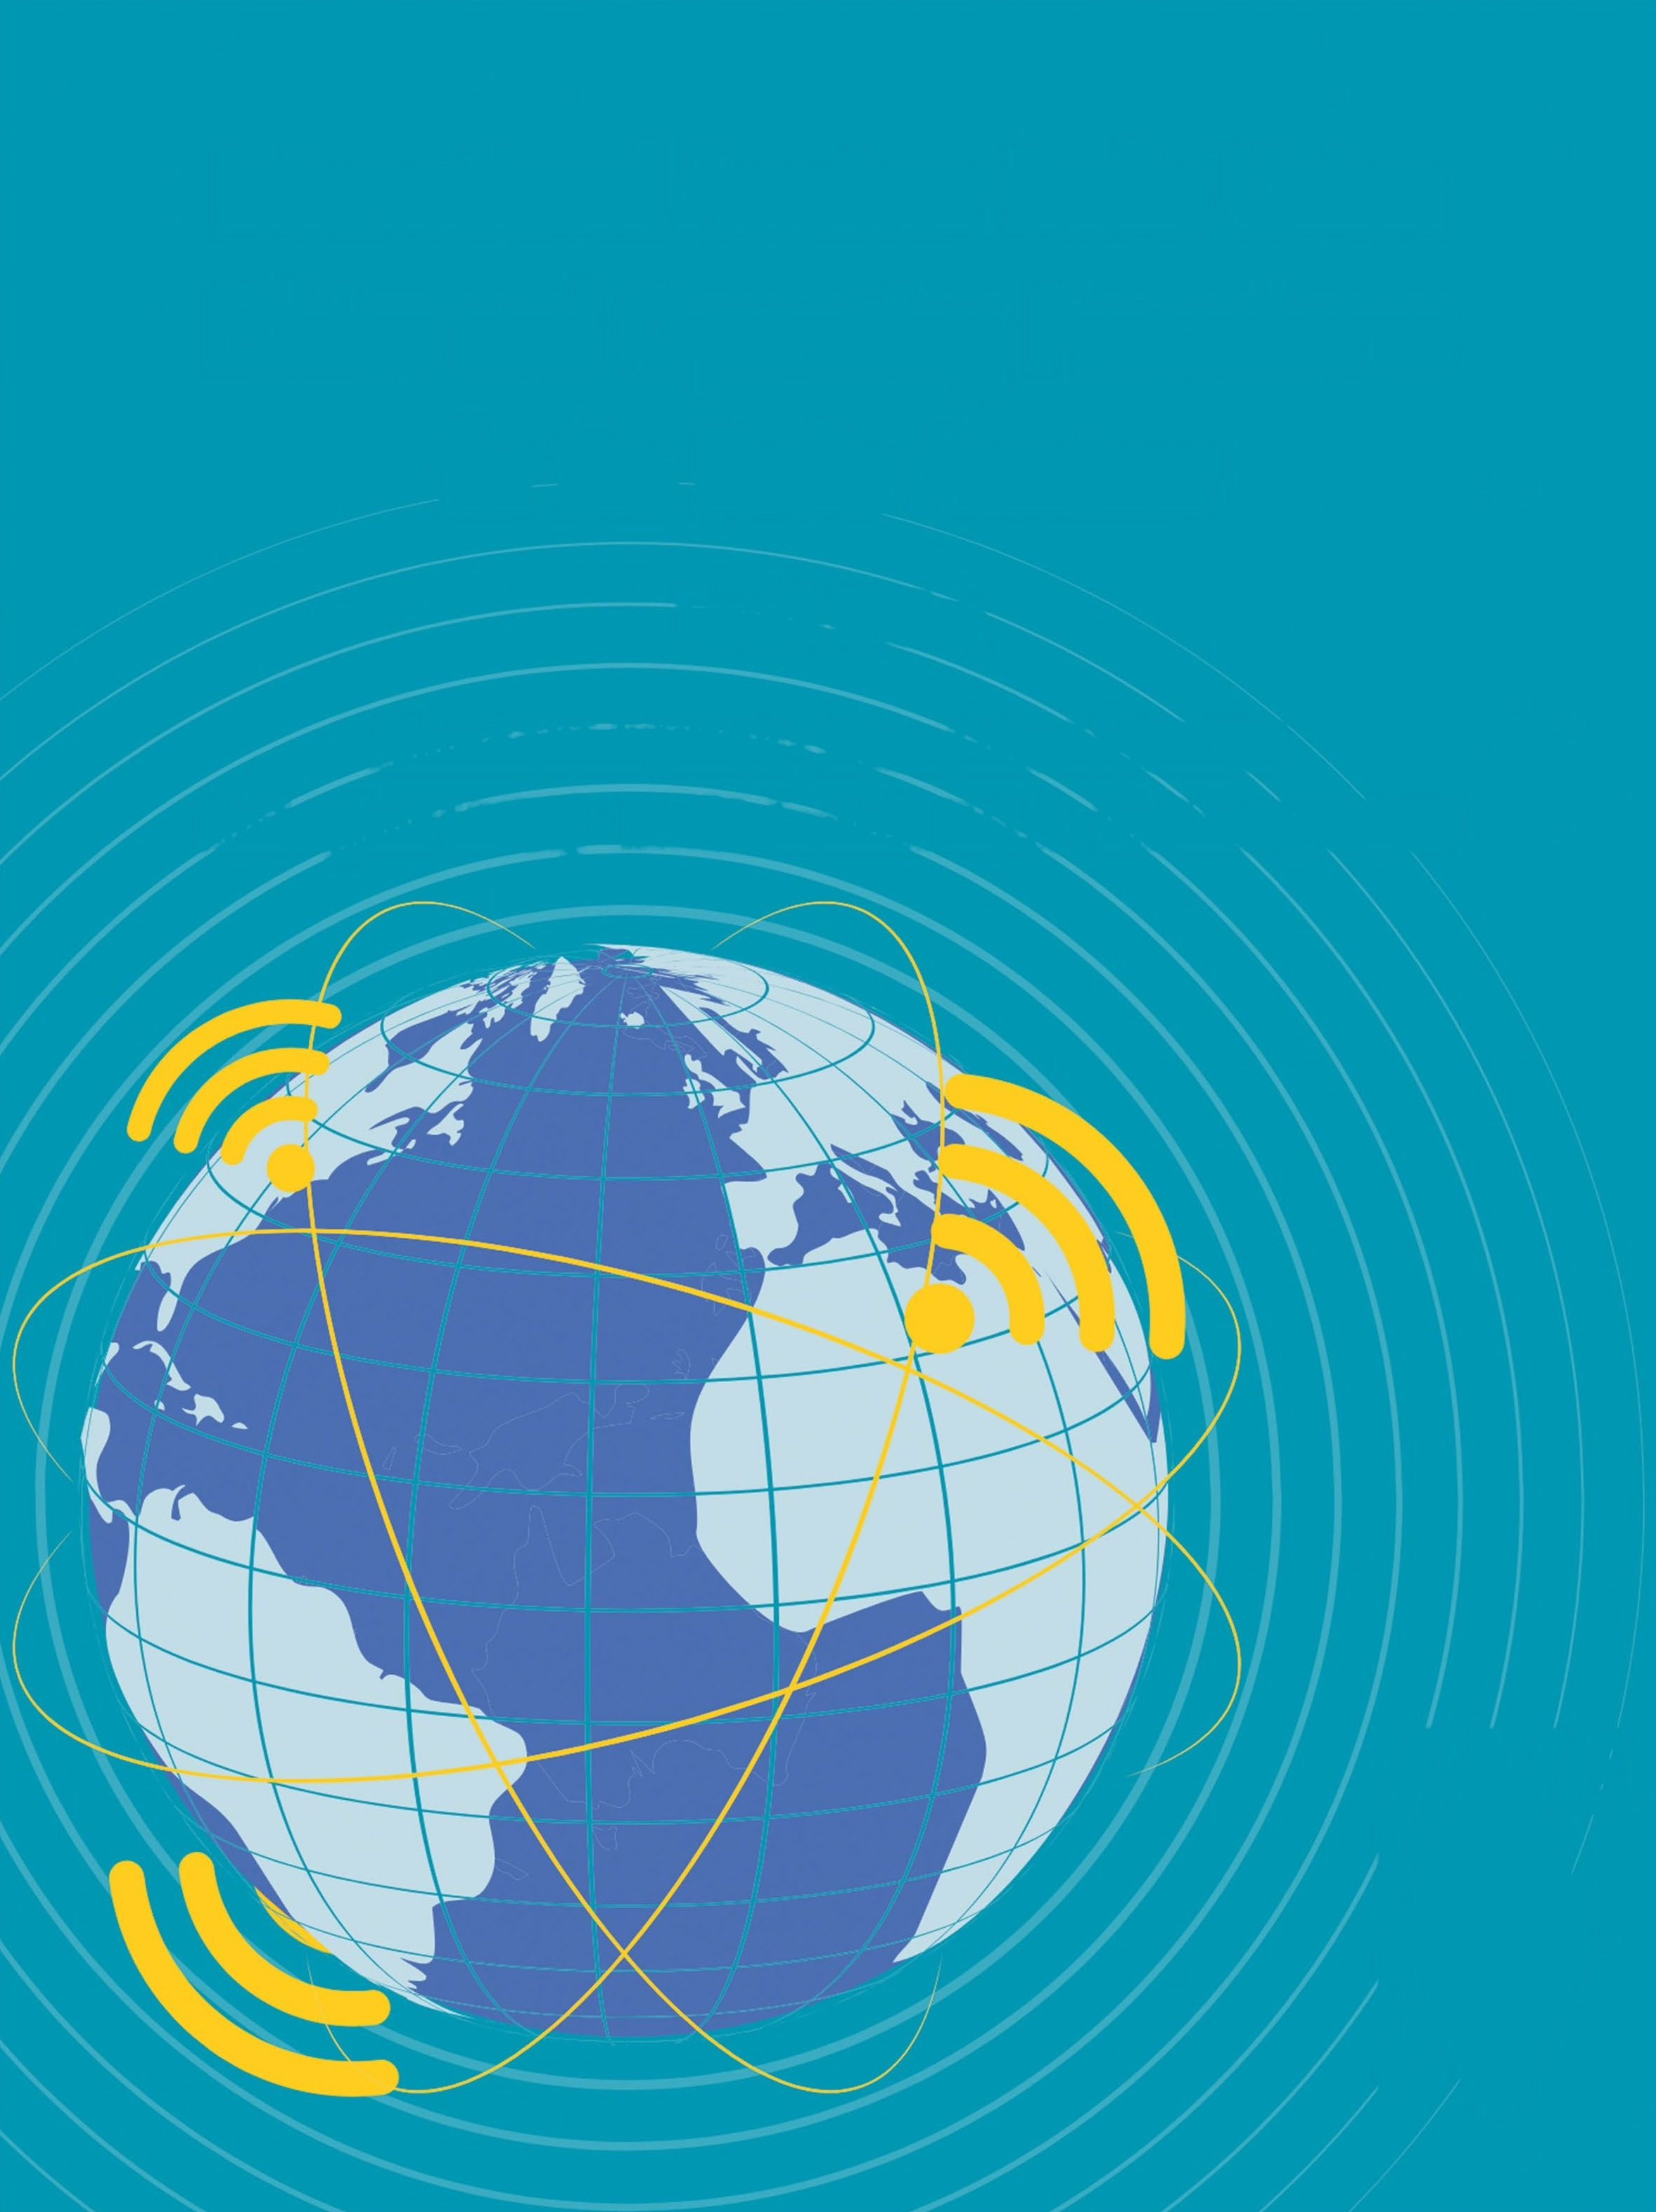
\includegraphics[height=246mm]{img/cover-clean.jpg}};
  \end{scope}
  % titolo
  \node[anchor=north,text width=\tw mm,align=center,inner sep=0pt]
    at ([xshift=\xc mm,yshift=246mm-20mm]O)
    {\color{eopcream}{\eopcoverreg\fontsize{19}{24}\selectfont International Amateur Radio Union\par}
     \vspace{3mm}{\eopcoverbold\fontsize{28}{33}\selectfont Etica e procedure operative\\per il radioamatore\par}
     \vspace{5mm}{\eopcoverreg\fontsize{14}{17}\selectfont Quarta edizione\par}
     \vspace{4mm}{\eopcoverreg\fontsize{10.5}{15}\selectfont
       Ahmad AlHoli 9K2DB · Marco Colombo IU2DXF\\
       Frode Igland LA6VQ · Rafal Lukawiecki EI6LA · Ian Suart GM4AUP\par}};
  % riquadro "non ufficiale"
  \node[anchor=south east,draw=eopcream,line width=0.8pt,rounded corners=3pt,
        fill=eopteal!85!black,inner xsep=8pt,inner ysep=6pt,text width=36mm,align=center]
    at ([xshift=\xr mm-13mm,yshift=15mm]O)
    {\color{eopcream}\sffamily\fontsize{8}{10.5}\selectfont
     \textbf{TRADUZIONE ITALIANA\\NON UFFICIALE}\\[2pt]
     per uso personale\\non approvata dall'IARU\\né dall'ARI};
  % ---- dorso: testo dal basso verso l'alto, solo se c'è spazio ----
  \pgfmathsetmacro\eopspinefs{min(11,1.4*\eopspine)}
  \ifdim\eopspine mm>3.9mm
    \node[rotate=90,inner sep=0pt,anchor=center]
      at ([xshift=\xs mm+0.5*\S mm,yshift=123mm]O)
      {\color{eopcream}\fontsize{\eopspinefs}{\eopspinefs}\selectfont
       {\eopcoverbold Etica e procedure operative per il radioamatore}%
       \hspace{0.9em}{\eopcoverreg IARU · Quarta edizione}};
  \fi
  % ---- quarta di copertina ----
  \node[anchor=north west,text width=\bw mm,inner sep=0pt]
    at ([xshift=21mm,yshift=246mm-25mm]O)
    {\eopnohyph\color{eopcream}
     {\eopcoverbold\fontsize{16.5}{20}\selectfont Etica e procedure operative per il radioamatore\par}
     \vspace{1.5mm}{\eopcoverreg\fontsize{11}{14}\selectfont Quarta edizione · traduzione italiana non ufficiale\par}
     \vspace{5mm}{\color{eopcream}\rule{25mm}{0.8pt}}\par
     \vspace{5mm}{\eopcoverreg\fontsize{10.5}{15.5}\selectfont
     Il riferimento dell'IARU su come comportarsi in aria: ascoltare prima di trasmettere,
     condurre un QSO in fonia, in CW e nei modi digitali, partecipare a pileup e contest,
     rispettare i piani di banda e convivere con gli altri utenti dello spettro radio.\par}};
  \node[anchor=south west,text width=\bw mm,inner sep=0pt]
    at ([xshift=21mm,yshift=24mm]O)
    {\eopnohyph\color{eopcream}\eopcoverreg\fontsize{8.5}{12}\selectfont
     Traduzione italiana non ufficiale di \emph{Ethics and Operating Procedures for the Radio Amateur},
     Fourth Edition, Revision~4.2.0, © 2026 International Amateur Radio Union Region~1,
     con licenza CC~BY-SA~4.0.\par
     \vspace{2.5mm}Non approvata dall'IARU né certificata dall'ARI. In caso di differenze fa fede l'edizione inglese.\par
     \vspace{2.5mm}github.com/BBerry2020/iaru-eop-it\par};
  % ---- linee guida (solo per l'anteprima, mai nel file di stampa) ----
  \ifnum\eopguides=1
    \draw[red,line width=0.3pt] ([xshift=3mm,yshift=3mm]O) rectangle ([xshift=\xr mm-3mm,yshift=243mm]O);
    \draw[red,dashed,line width=0.3pt] ([xshift=\xs mm]O) -- ([xshift=\xs mm,yshift=246mm]O)
      ([xshift=\xf mm]O) -- ([xshift=\xf mm,yshift=246mm]O);
  \fi
\end{tikzpicture}
\null
% seconda pagina: 2ª e 3ª di copertina (interno), lasciate bianche come chiede 4graph
\newpage
\null
\end{document}
"
% (senza \def: 165 mm di larghezza, 240 mm di altezza, dorso 5,5 mm).
\ifdefined\eoptrimw\else\def\eoptrimw{165}\fi
\ifdefined\eopspine\else\def\eopspine{5.5}\fi
\ifdefined\eopguides\else\def\eopguides{0}\fi
\newdimen\eoppw \eoppw=\dimexpr 2\dimexpr\eoptrimw mm\relax+6mm+\eopspine mm\relax
\documentclass{article}
\usepackage{fontspec}
\defaultfontfeatures{Ligatures=TeX}% apostrofi tipografici ’
\usepackage{tikz}
\usepackage{xcolor}
\usepackage[paperwidth=\the\eoppw,paperheight=246mm,margin=0pt]{geometry}
\pagestyle{empty}
\frenchspacing
\setlength{\parindent}{0pt}
\newfontfamily\eopcoverfont{SourceSans3}[Path=fonts/,Extension=.otf,UprightFont=*-Light,BoldFont=*-Regular,WordSpace={1.9,1.4,1}]
\setsansfont{SourceSans3}[Path=fonts/,Extension=.otf,
  UprightFont=*-Regular,ItalicFont=*-It,BoldFont=*-Semibold,BoldItalicFont=*-SemiboldIt]
\newfontfamily\eopcoverbold{SourceSans3}[Path=fonts/,Extension=.otf,UprightFont=*-Semibold,WordSpace=1.3]
\newfontfamily\eopcoverreg{SourceSans3}[Path=fonts/,Extension=.otf,UprightFont=*-Regular,ItalicFont=*-It]
% testo della copertina: niente sillabazione, righe a bandiera
\newcommand{\eopnohyph}{\hyphenpenalty=10000 \exhyphenpenalty=10000 \raggedright}
% colori in RGB: Ghostscript li converte in CMYK FOGRA51 insieme all'immagine,
% così fondo e foto finiscono con gli stessi valori di inchiostro
\definecolor{eopteal}{HTML}{0097B2}
\definecolor{eopcream}{HTML}{FCE8A2}

\begin{document}
\begin{tikzpicture}[remember picture,overlay,x=1mm,y=1mm]
  % origine: angolo in basso a sinistra del foglio (abbondanza compresa)
  \coordinate (O) at (current page.south west);
  \def\S{\eopspine}
  \pgfmathsetmacro\xs{\eoptrimw+3}               % piega quarta/dorso
  \pgfmathsetmacro\xf{\eoptrimw+3+\eopspine}     % piega dorso/prima
  \pgfmathsetmacro\xc{\xf+\eoptrimw/2}           % centro della prima
  \pgfmathsetmacro\xr{2*\eoptrimw+6+\eopspine}   % bordo destro del foglio
  \pgfmathsetmacro\tw{\eoptrimw-24}              % giustezza del titolo in prima (12 mm dai bordi)
  \pgfmathsetmacro\bw{\eoptrimw-36}              % giustezza dei testi in quarta
  % ---- fondo azzurro: quarta e dorso ----
  \fill[eopteal] (O) rectangle ([xshift=\xf mm+4mm,yshift=246mm]O);
  % ---- prima di copertina: immagine centrata sul rifilo, tagliata ai lati ----
  \begin{scope}
    \clip ([xshift=\xf mm]O) rectangle ([xshift=\xr mm,yshift=246mm]O);
    % immagine allineata alla piega del dorso (il globo resta ad almeno 10 mm), tagliata a destra
    \node[inner sep=0pt,anchor=west] at ([xshift=\xf mm+3mm,yshift=123mm]O)
      {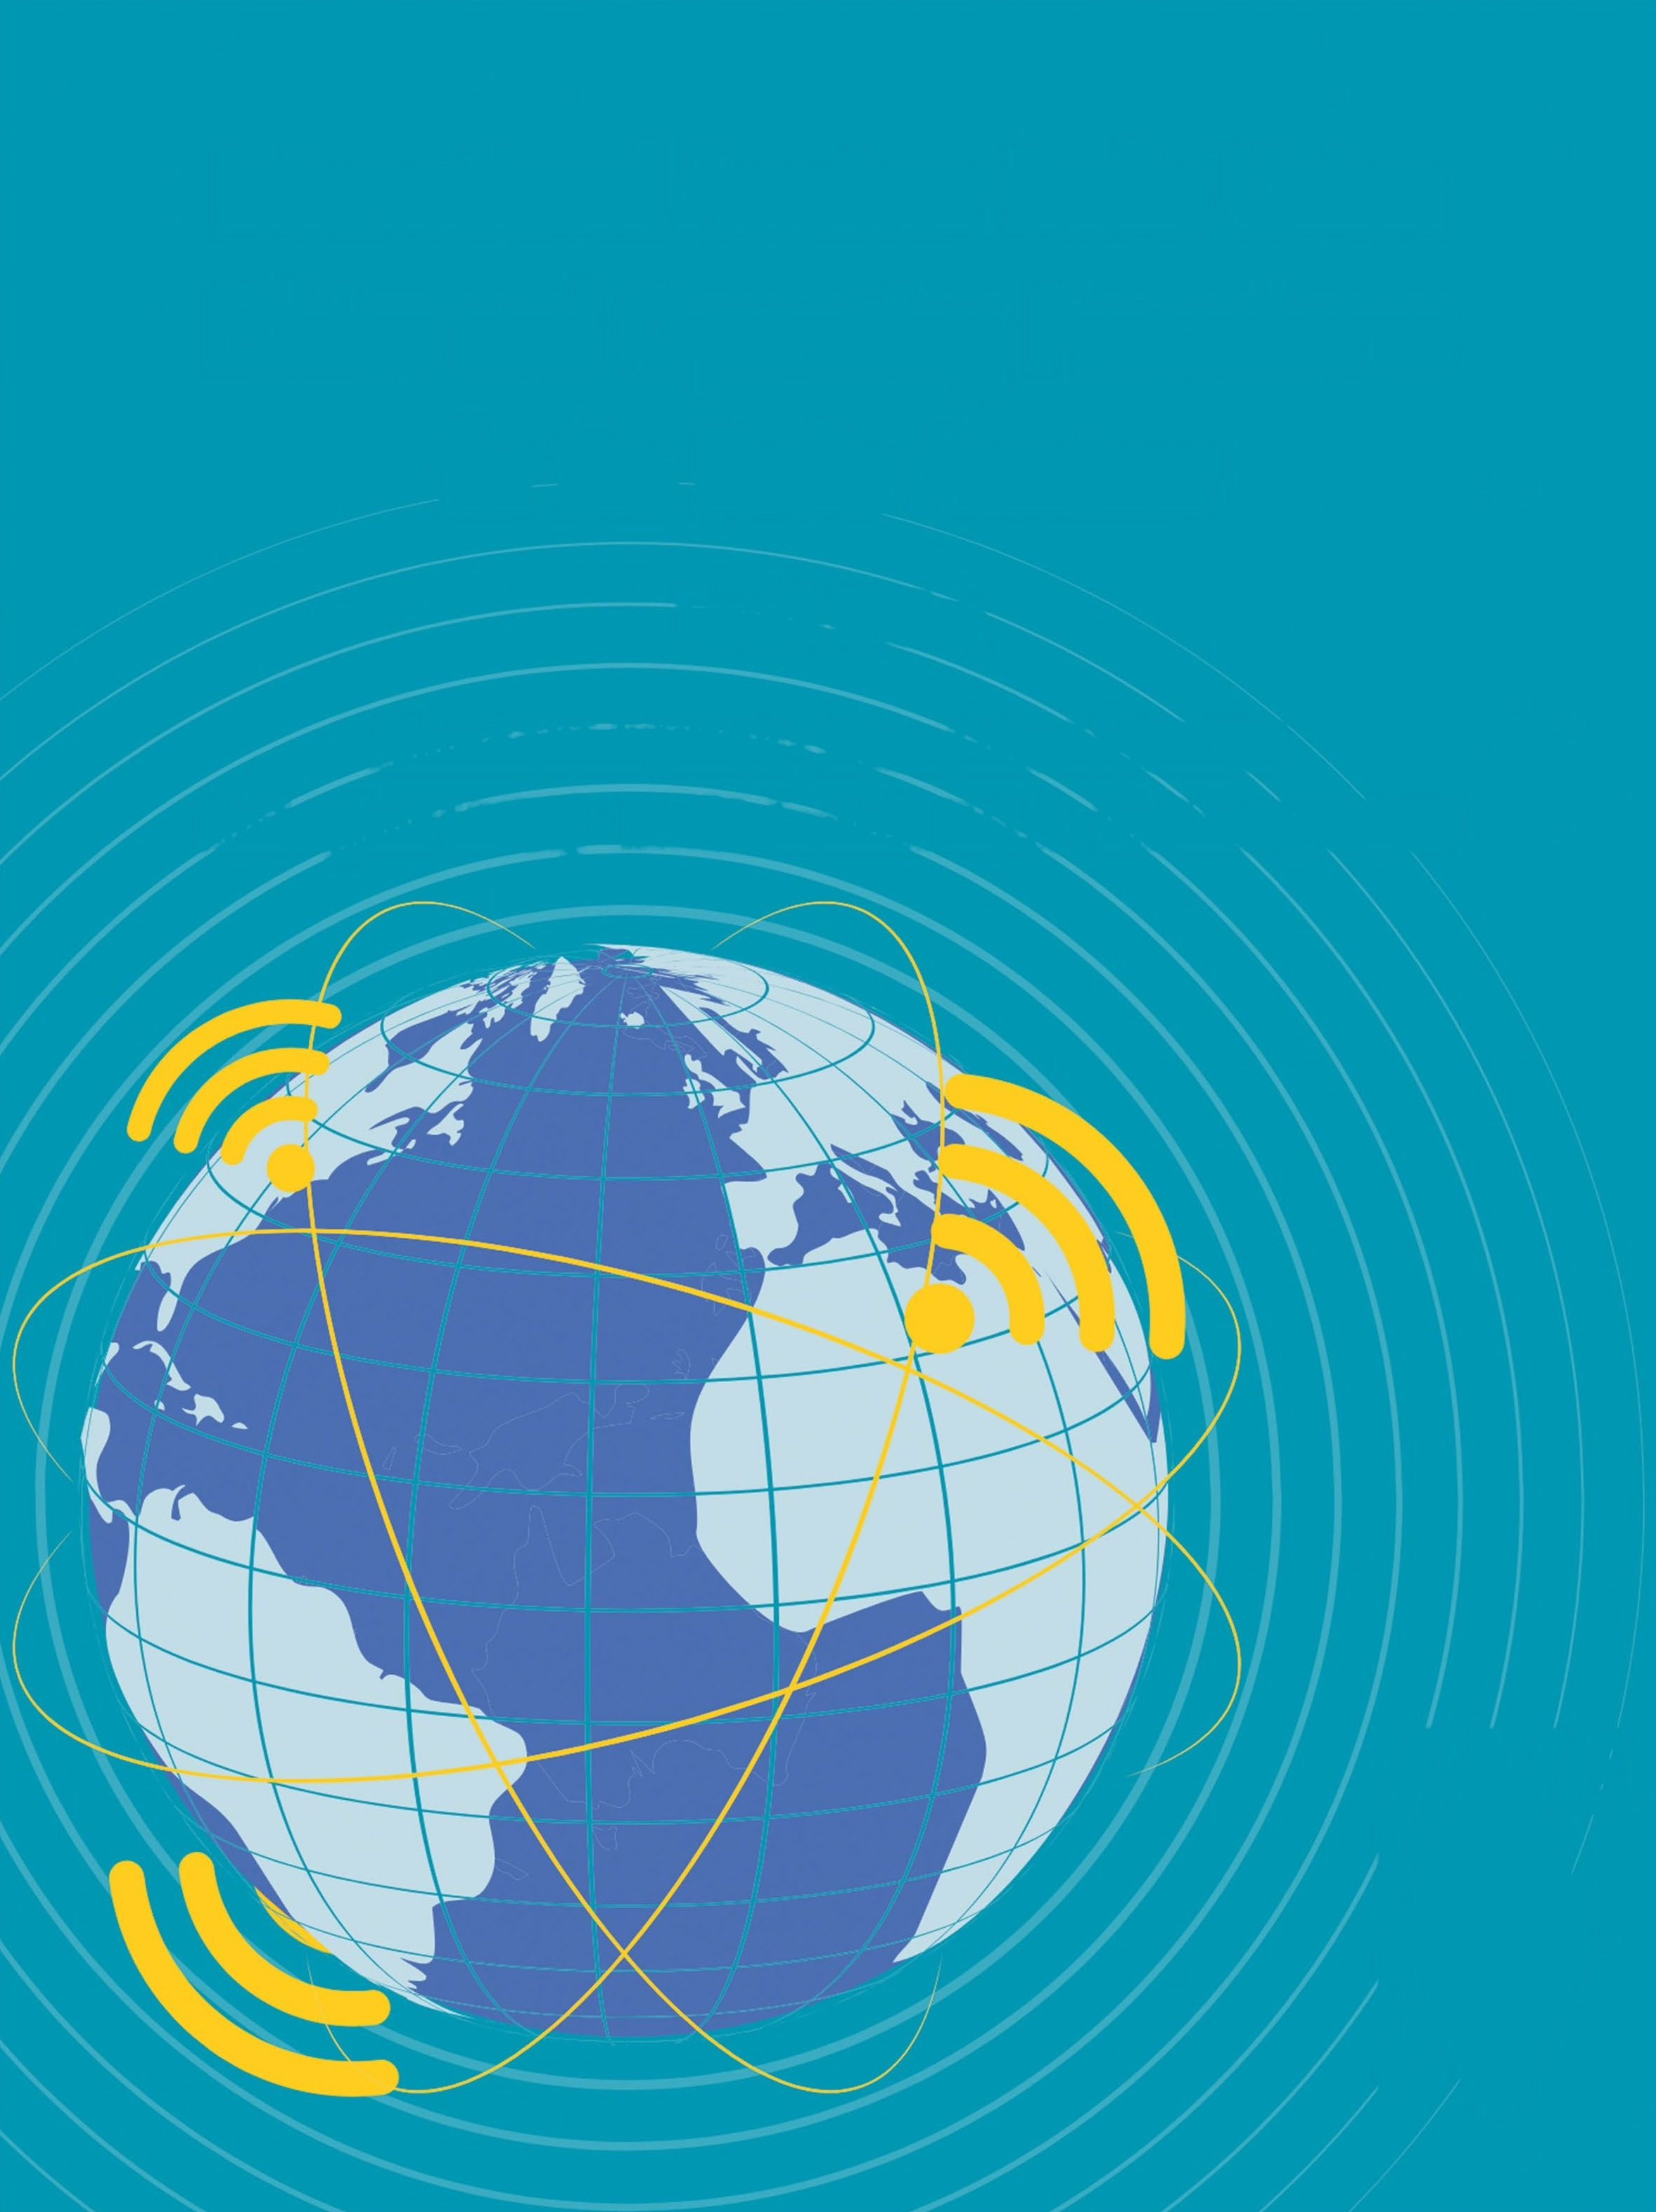
\includegraphics[height=246mm]{img/cover-clean.jpg}};
  \end{scope}
  % titolo
  \node[anchor=north,text width=\tw mm,align=center,inner sep=0pt]
    at ([xshift=\xc mm,yshift=246mm-20mm]O)
    {\color{eopcream}{\eopcoverreg\fontsize{19}{24}\selectfont International Amateur Radio Union\par}
     \vspace{3mm}{\eopcoverbold\fontsize{28}{33}\selectfont Etica e procedure operative\\per il radioamatore\par}
     \vspace{5mm}{\eopcoverreg\fontsize{14}{17}\selectfont Quarta edizione\par}
     \vspace{4mm}{\eopcoverreg\fontsize{10.5}{15}\selectfont
       Ahmad AlHoli 9K2DB · Marco Colombo IU2DXF\\
       Frode Igland LA6VQ · Rafal Lukawiecki EI6LA · Ian Suart GM4AUP\par}};
  % riquadro "non ufficiale"
  \node[anchor=south east,draw=eopcream,line width=0.8pt,rounded corners=3pt,
        fill=eopteal!85!black,inner xsep=8pt,inner ysep=6pt,text width=36mm,align=center]
    at ([xshift=\xr mm-13mm,yshift=15mm]O)
    {\color{eopcream}\sffamily\fontsize{8}{10.5}\selectfont
     \textbf{TRADUZIONE ITALIANA\\NON UFFICIALE}\\[2pt]
     per uso personale\\non approvata dall'IARU\\né dall'ARI};
  % ---- dorso: testo dal basso verso l'alto, solo se c'è spazio ----
  \pgfmathsetmacro\eopspinefs{min(11,1.4*\eopspine)}
  \ifdim\eopspine mm>3.9mm
    \node[rotate=90,inner sep=0pt,anchor=center]
      at ([xshift=\xs mm+0.5*\S mm,yshift=123mm]O)
      {\color{eopcream}\fontsize{\eopspinefs}{\eopspinefs}\selectfont
       {\eopcoverbold Etica e procedure operative per il radioamatore}%
       \hspace{0.9em}{\eopcoverreg IARU · Quarta edizione}};
  \fi
  % ---- quarta di copertina ----
  \node[anchor=north west,text width=\bw mm,inner sep=0pt]
    at ([xshift=21mm,yshift=246mm-25mm]O)
    {\eopnohyph\color{eopcream}
     {\eopcoverbold\fontsize{16.5}{20}\selectfont Etica e procedure operative per il radioamatore\par}
     \vspace{1.5mm}{\eopcoverreg\fontsize{11}{14}\selectfont Quarta edizione · traduzione italiana non ufficiale\par}
     \vspace{5mm}{\color{eopcream}\rule{25mm}{0.8pt}}\par
     \vspace{5mm}{\eopcoverreg\fontsize{10.5}{15.5}\selectfont
     Il riferimento dell'IARU su come comportarsi in aria: ascoltare prima di trasmettere,
     condurre un QSO in fonia, in CW e nei modi digitali, partecipare a pileup e contest,
     rispettare i piani di banda e convivere con gli altri utenti dello spettro radio.\par}};
  \node[anchor=south west,text width=\bw mm,inner sep=0pt]
    at ([xshift=21mm,yshift=24mm]O)
    {\eopnohyph\color{eopcream}\eopcoverreg\fontsize{8.5}{12}\selectfont
     Traduzione italiana non ufficiale di \emph{Ethics and Operating Procedures for the Radio Amateur},
     Fourth Edition, Revision~4.2.0, © 2026 International Amateur Radio Union Region~1,
     con licenza CC~BY-SA~4.0.\par
     \vspace{2.5mm}Non approvata dall'IARU né certificata dall'ARI. In caso di differenze fa fede l'edizione inglese.\par
     \vspace{2.5mm}github.com/BBerry2020/iaru-eop-it\par};
  % ---- linee guida (solo per l'anteprima, mai nel file di stampa) ----
  \ifnum\eopguides=1
    \draw[red,line width=0.3pt] ([xshift=3mm,yshift=3mm]O) rectangle ([xshift=\xr mm-3mm,yshift=243mm]O);
    \draw[red,dashed,line width=0.3pt] ([xshift=\xs mm]O) -- ([xshift=\xs mm,yshift=246mm]O)
      ([xshift=\xf mm]O) -- ([xshift=\xf mm,yshift=246mm]O);
  \fi
\end{tikzpicture}
\null
% seconda pagina: 2ª e 3ª di copertina (interno), lasciate bianche come chiede 4graph
\newpage
\null
\end{document}
"
% (senza \def: 165 mm di larghezza, 240 mm di altezza, dorso 5,5 mm).
\ifdefined\eoptrimw\else\def\eoptrimw{165}\fi
\ifdefined\eopspine\else\def\eopspine{5.5}\fi
\ifdefined\eopguides\else\def\eopguides{0}\fi
\newdimen\eoppw \eoppw=\dimexpr 2\dimexpr\eoptrimw mm\relax+6mm+\eopspine mm\relax
\documentclass{article}
\usepackage{fontspec}
\defaultfontfeatures{Ligatures=TeX}% apostrofi tipografici ’
\usepackage{tikz}
\usepackage{xcolor}
\usepackage[paperwidth=\the\eoppw,paperheight=246mm,margin=0pt]{geometry}
\pagestyle{empty}
\frenchspacing
\setlength{\parindent}{0pt}
\newfontfamily\eopcoverfont{SourceSans3}[Path=fonts/,Extension=.otf,UprightFont=*-Light,BoldFont=*-Regular,WordSpace={1.9,1.4,1}]
\setsansfont{SourceSans3}[Path=fonts/,Extension=.otf,
  UprightFont=*-Regular,ItalicFont=*-It,BoldFont=*-Semibold,BoldItalicFont=*-SemiboldIt]
\newfontfamily\eopcoverbold{SourceSans3}[Path=fonts/,Extension=.otf,UprightFont=*-Semibold,WordSpace=1.3]
\newfontfamily\eopcoverreg{SourceSans3}[Path=fonts/,Extension=.otf,UprightFont=*-Regular,ItalicFont=*-It]
% testo della copertina: niente sillabazione, righe a bandiera
\newcommand{\eopnohyph}{\hyphenpenalty=10000 \exhyphenpenalty=10000 \raggedright}
% colori in RGB: Ghostscript li converte in CMYK FOGRA51 insieme all'immagine,
% così fondo e foto finiscono con gli stessi valori di inchiostro
\definecolor{eopteal}{HTML}{0097B2}
\definecolor{eopcream}{HTML}{FCE8A2}

\begin{document}
\begin{tikzpicture}[remember picture,overlay,x=1mm,y=1mm]
  % origine: angolo in basso a sinistra del foglio (abbondanza compresa)
  \coordinate (O) at (current page.south west);
  \def\S{\eopspine}
  \pgfmathsetmacro\xs{\eoptrimw+3}               % piega quarta/dorso
  \pgfmathsetmacro\xf{\eoptrimw+3+\eopspine}     % piega dorso/prima
  \pgfmathsetmacro\xc{\xf+\eoptrimw/2}           % centro della prima
  \pgfmathsetmacro\xr{2*\eoptrimw+6+\eopspine}   % bordo destro del foglio
  \pgfmathsetmacro\tw{\eoptrimw-24}              % giustezza del titolo in prima (12 mm dai bordi)
  \pgfmathsetmacro\bw{\eoptrimw-36}              % giustezza dei testi in quarta
  % ---- fondo azzurro: quarta e dorso ----
  \fill[eopteal] (O) rectangle ([xshift=\xf mm+4mm,yshift=246mm]O);
  % ---- prima di copertina: immagine centrata sul rifilo, tagliata ai lati ----
  \begin{scope}
    \clip ([xshift=\xf mm]O) rectangle ([xshift=\xr mm,yshift=246mm]O);
    % immagine allineata alla piega del dorso (il globo resta ad almeno 10 mm), tagliata a destra
    \node[inner sep=0pt,anchor=west] at ([xshift=\xf mm+3mm,yshift=123mm]O)
      {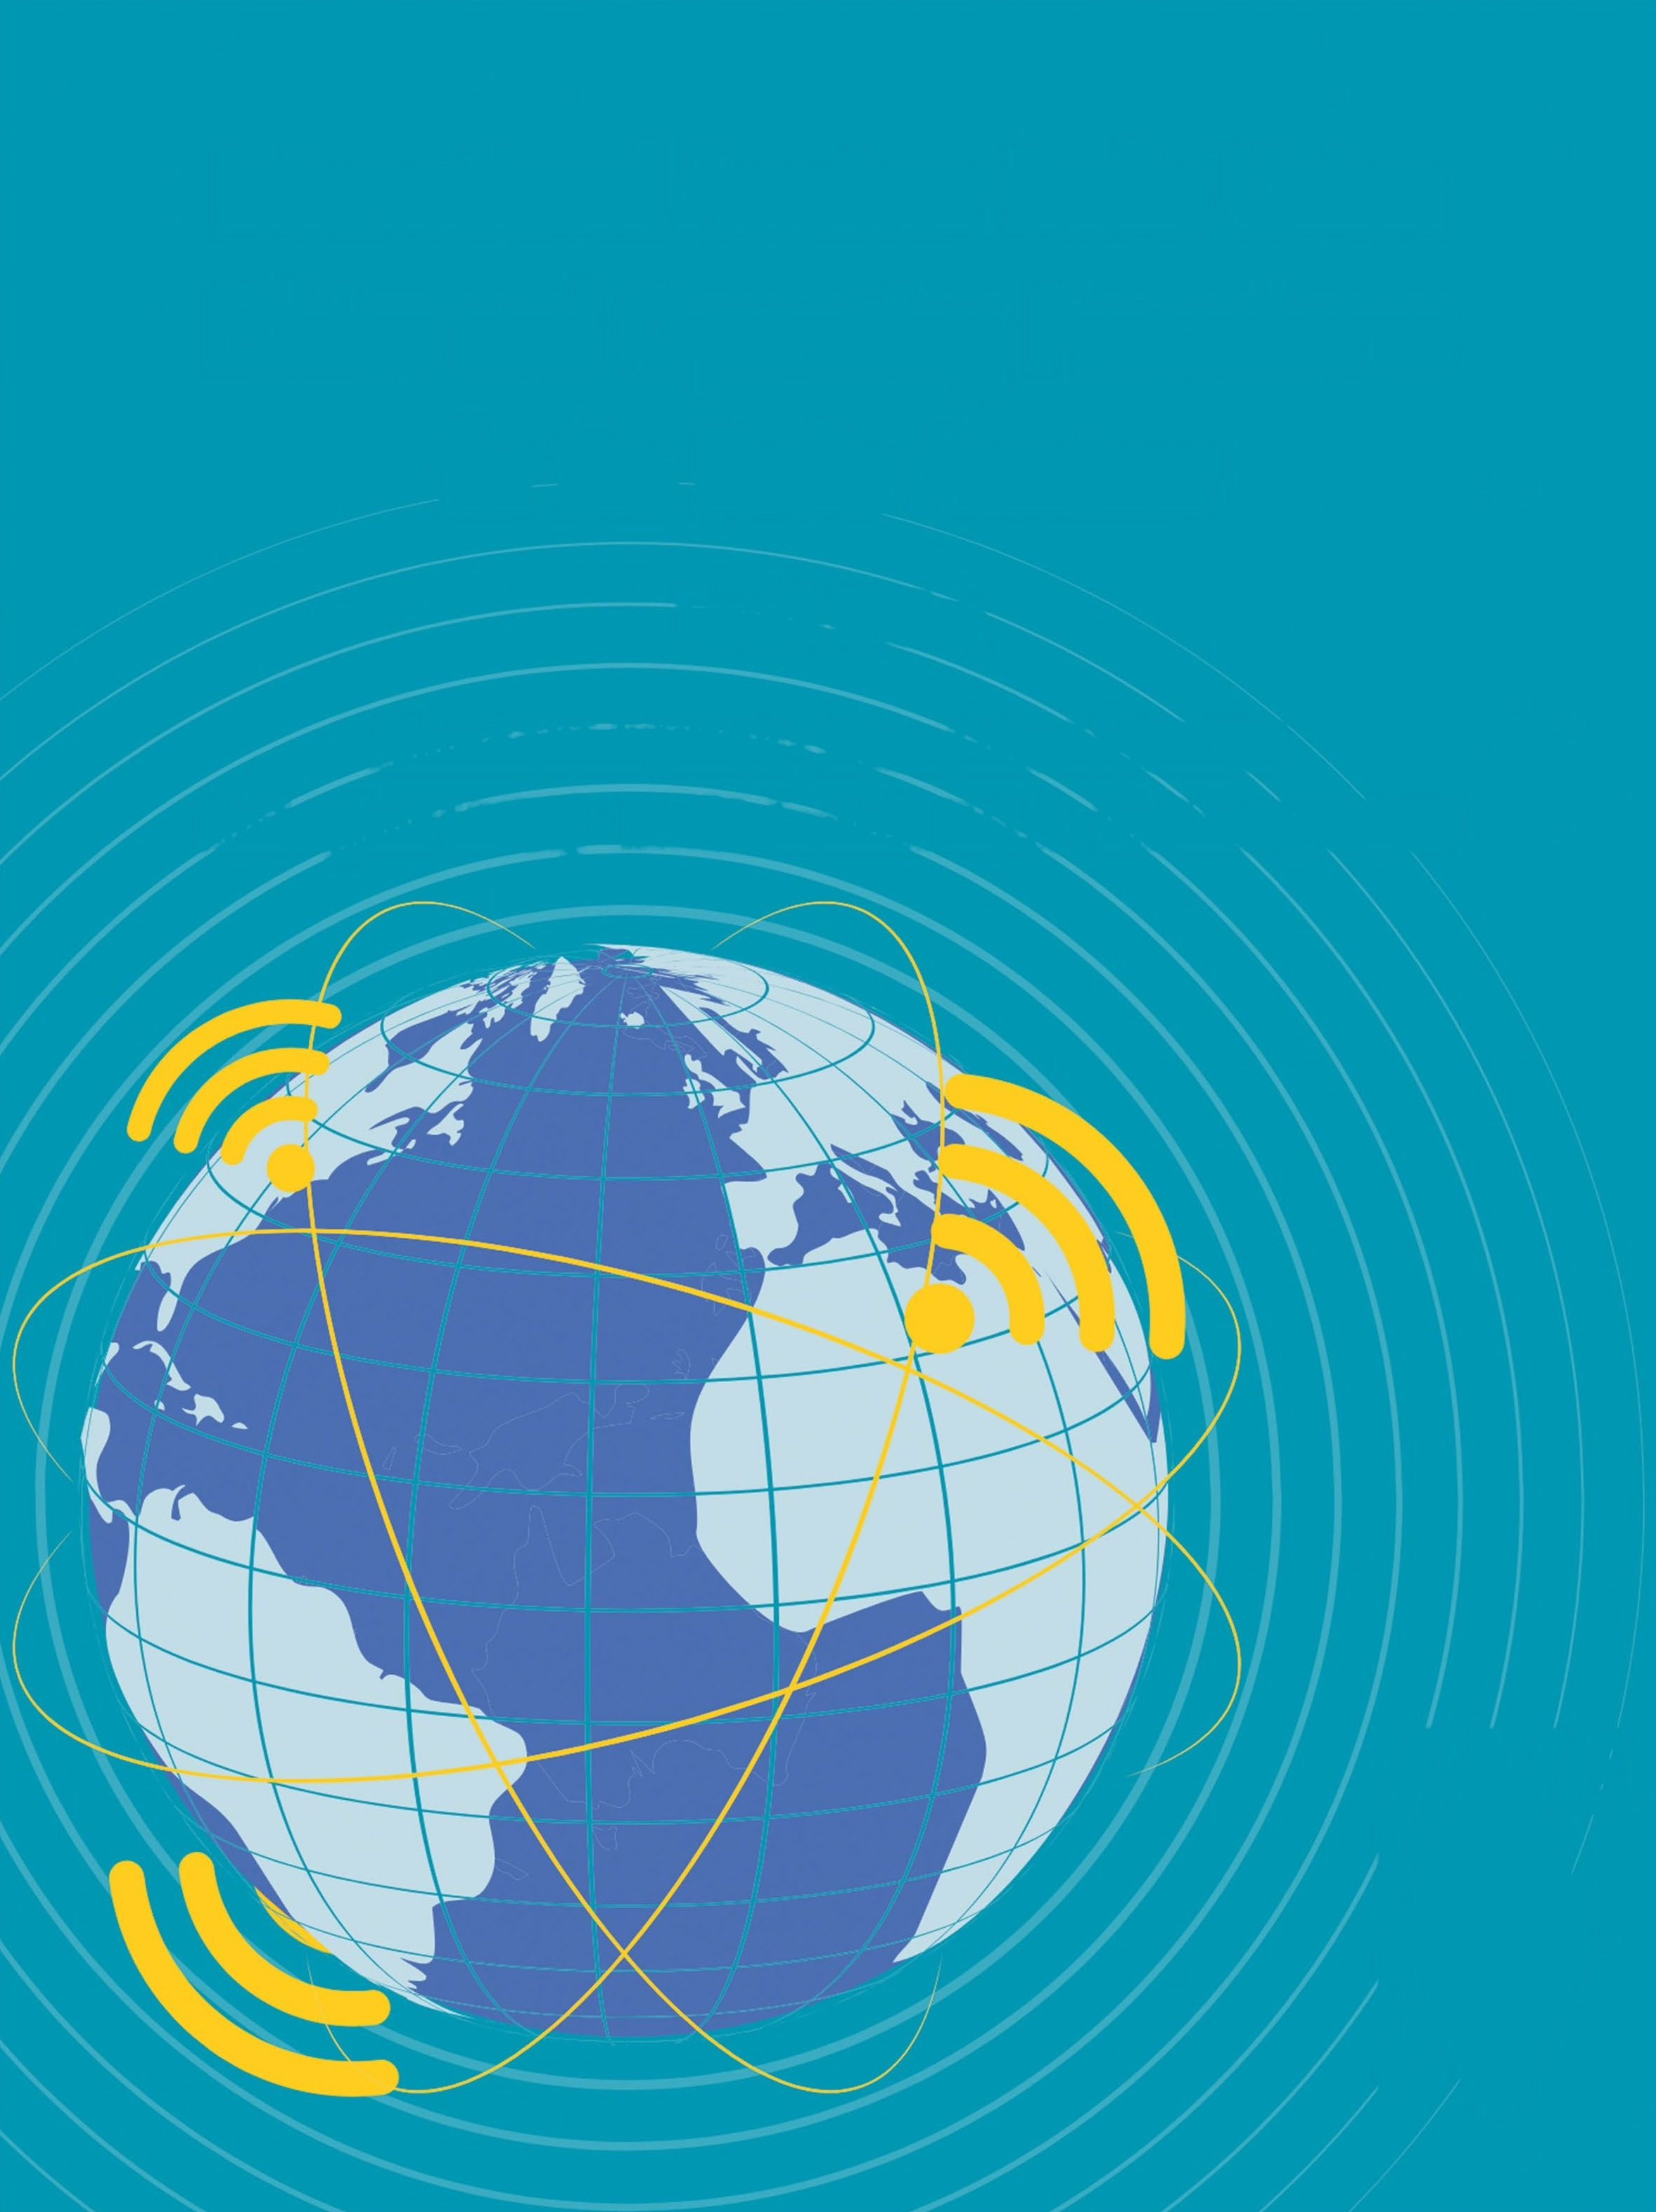
\includegraphics[height=246mm]{img/cover-clean.jpg}};
  \end{scope}
  % titolo
  \node[anchor=north,text width=\tw mm,align=center,inner sep=0pt]
    at ([xshift=\xc mm,yshift=246mm-20mm]O)
    {\color{eopcream}{\eopcoverreg\fontsize{19}{24}\selectfont International Amateur Radio Union\par}
     \vspace{3mm}{\eopcoverbold\fontsize{28}{33}\selectfont Etica e procedure operative\\per il radioamatore\par}
     \vspace{5mm}{\eopcoverreg\fontsize{14}{17}\selectfont Quarta edizione\par}
     \vspace{4mm}{\eopcoverreg\fontsize{10.5}{15}\selectfont
       Ahmad AlHoli 9K2DB · Marco Colombo IU2DXF\\
       Frode Igland LA6VQ · Rafal Lukawiecki EI6LA · Ian Suart GM4AUP\par}};
  % riquadro "non ufficiale"
  \node[anchor=south east,draw=eopcream,line width=0.8pt,rounded corners=3pt,
        fill=eopteal!85!black,inner xsep=8pt,inner ysep=6pt,text width=36mm,align=center]
    at ([xshift=\xr mm-13mm,yshift=15mm]O)
    {\color{eopcream}\sffamily\fontsize{8}{10.5}\selectfont
     \textbf{TRADUZIONE ITALIANA\\NON UFFICIALE}\\[2pt]
     per uso personale\\non approvata dall'IARU\\né dall'ARI};
  % ---- dorso: testo dal basso verso l'alto, solo se c'è spazio ----
  \pgfmathsetmacro\eopspinefs{min(11,1.4*\eopspine)}
  \ifdim\eopspine mm>3.9mm
    \node[rotate=90,inner sep=0pt,anchor=center]
      at ([xshift=\xs mm+0.5*\S mm,yshift=123mm]O)
      {\color{eopcream}\fontsize{\eopspinefs}{\eopspinefs}\selectfont
       {\eopcoverbold Etica e procedure operative per il radioamatore}%
       \hspace{0.9em}{\eopcoverreg IARU · Quarta edizione}};
  \fi
  % ---- quarta di copertina ----
  \node[anchor=north west,text width=\bw mm,inner sep=0pt]
    at ([xshift=21mm,yshift=246mm-25mm]O)
    {\eopnohyph\color{eopcream}
     {\eopcoverbold\fontsize{16.5}{20}\selectfont Etica e procedure operative per il radioamatore\par}
     \vspace{1.5mm}{\eopcoverreg\fontsize{11}{14}\selectfont Quarta edizione · traduzione italiana non ufficiale\par}
     \vspace{5mm}{\color{eopcream}\rule{25mm}{0.8pt}}\par
     \vspace{5mm}{\eopcoverreg\fontsize{10.5}{15.5}\selectfont
     Il riferimento dell'IARU su come comportarsi in aria: ascoltare prima di trasmettere,
     condurre un QSO in fonia, in CW e nei modi digitali, partecipare a pileup e contest,
     rispettare i piani di banda e convivere con gli altri utenti dello spettro radio.\par}};
  \node[anchor=south west,text width=\bw mm,inner sep=0pt]
    at ([xshift=21mm,yshift=24mm]O)
    {\eopnohyph\color{eopcream}\eopcoverreg\fontsize{8.5}{12}\selectfont
     Traduzione italiana non ufficiale di \emph{Ethics and Operating Procedures for the Radio Amateur},
     Fourth Edition, Revision~4.2.0, © 2026 International Amateur Radio Union Region~1,
     con licenza CC~BY-SA~4.0.\par
     \vspace{2.5mm}Non approvata dall'IARU né certificata dall'ARI. In caso di differenze fa fede l'edizione inglese.\par
     \vspace{2.5mm}github.com/BBerry2020/iaru-eop-it\par};
  % ---- linee guida (solo per l'anteprima, mai nel file di stampa) ----
  \ifnum\eopguides=1
    \draw[red,line width=0.3pt] ([xshift=3mm,yshift=3mm]O) rectangle ([xshift=\xr mm-3mm,yshift=243mm]O);
    \draw[red,dashed,line width=0.3pt] ([xshift=\xs mm]O) -- ([xshift=\xs mm,yshift=246mm]O)
      ([xshift=\xf mm]O) -- ([xshift=\xf mm,yshift=246mm]O);
  \fi
\end{tikzpicture}
\null
% seconda pagina: 2ª e 3ª di copertina (interno), lasciate bianche come chiede 4graph
\newpage
\null
\end{document}
"
% (senza \def: 165 mm di larghezza, 240 mm di altezza, dorso 5,5 mm).
\ifdefined\eoptrimw\else\def\eoptrimw{165}\fi
\ifdefined\eopspine\else\def\eopspine{5.5}\fi
\ifdefined\eopguides\else\def\eopguides{0}\fi
\newdimen\eoppw \eoppw=\dimexpr 2\dimexpr\eoptrimw mm\relax+6mm+\eopspine mm\relax
\documentclass{article}
\usepackage{fontspec}
\defaultfontfeatures{Ligatures=TeX}% apostrofi tipografici ’
\usepackage{tikz}
\usepackage{xcolor}
\usepackage[paperwidth=\the\eoppw,paperheight=246mm,margin=0pt]{geometry}
\pagestyle{empty}
\frenchspacing
\setlength{\parindent}{0pt}
\newfontfamily\eopcoverfont{SourceSans3}[Path=fonts/,Extension=.otf,UprightFont=*-Light,BoldFont=*-Regular,WordSpace={1.9,1.4,1}]
\setsansfont{SourceSans3}[Path=fonts/,Extension=.otf,
  UprightFont=*-Regular,ItalicFont=*-It,BoldFont=*-Semibold,BoldItalicFont=*-SemiboldIt]
\newfontfamily\eopcoverbold{SourceSans3}[Path=fonts/,Extension=.otf,UprightFont=*-Semibold,WordSpace=1.3]
\newfontfamily\eopcoverreg{SourceSans3}[Path=fonts/,Extension=.otf,UprightFont=*-Regular,ItalicFont=*-It]
% testo della copertina: niente sillabazione, righe a bandiera
\newcommand{\eopnohyph}{\hyphenpenalty=10000 \exhyphenpenalty=10000 \raggedright}
% colori in RGB: Ghostscript li converte in CMYK FOGRA51 insieme all'immagine,
% così fondo e foto finiscono con gli stessi valori di inchiostro
\definecolor{eopteal}{HTML}{0097B2}
\definecolor{eopcream}{HTML}{FCE8A2}

\begin{document}
\begin{tikzpicture}[remember picture,overlay,x=1mm,y=1mm]
  % origine: angolo in basso a sinistra del foglio (abbondanza compresa)
  \coordinate (O) at (current page.south west);
  \def\S{\eopspine}
  \pgfmathsetmacro\xs{\eoptrimw+3}               % piega quarta/dorso
  \pgfmathsetmacro\xf{\eoptrimw+3+\eopspine}     % piega dorso/prima
  \pgfmathsetmacro\xc{\xf+\eoptrimw/2}           % centro della prima
  \pgfmathsetmacro\xr{2*\eoptrimw+6+\eopspine}   % bordo destro del foglio
  \pgfmathsetmacro\tw{\eoptrimw-24}              % giustezza del titolo in prima (12 mm dai bordi)
  \pgfmathsetmacro\bw{\eoptrimw-36}              % giustezza dei testi in quarta
  % ---- fondo azzurro: quarta e dorso ----
  \fill[eopteal] (O) rectangle ([xshift=\xf mm+4mm,yshift=246mm]O);
  % ---- prima di copertina: immagine centrata sul rifilo, tagliata ai lati ----
  \begin{scope}
    \clip ([xshift=\xf mm]O) rectangle ([xshift=\xr mm,yshift=246mm]O);
    % immagine allineata alla piega del dorso (il globo resta ad almeno 10 mm), tagliata a destra
    \node[inner sep=0pt,anchor=west] at ([xshift=\xf mm+3mm,yshift=123mm]O)
      {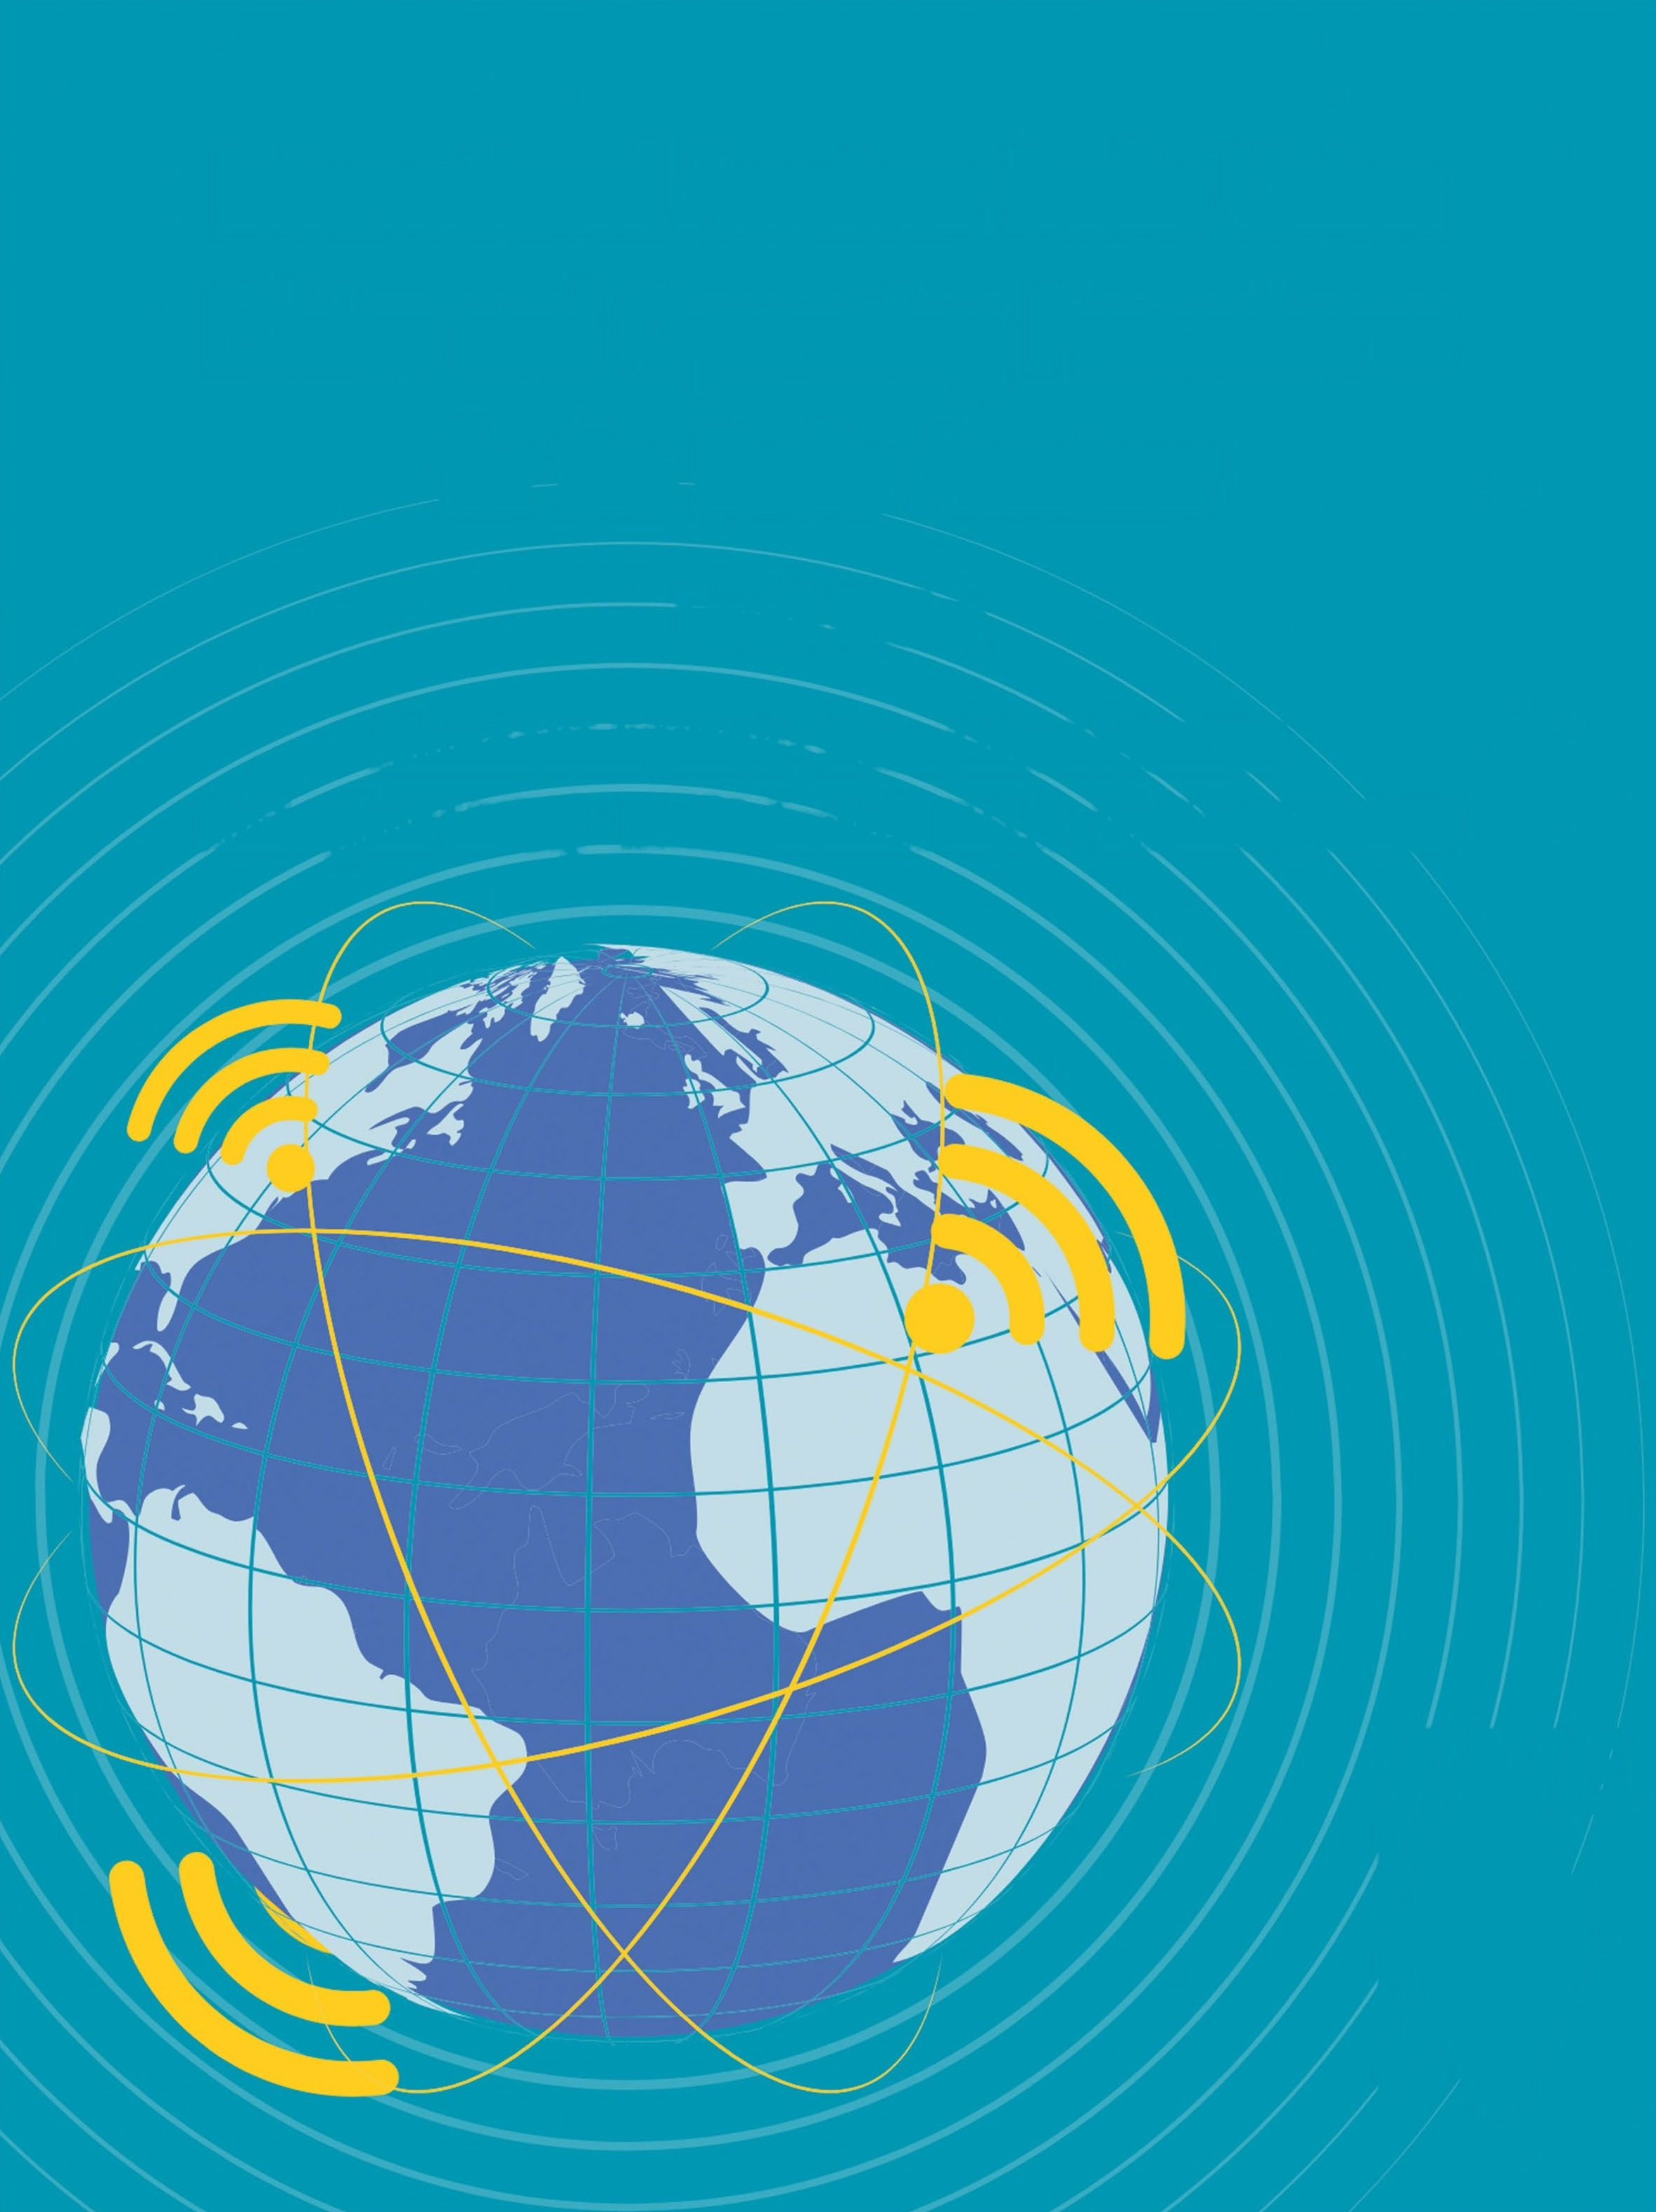
\includegraphics[height=246mm]{img/cover-clean.jpg}};
  \end{scope}
  % titolo
  \node[anchor=north,text width=\tw mm,align=center,inner sep=0pt]
    at ([xshift=\xc mm,yshift=246mm-20mm]O)
    {\color{eopcream}{\eopcoverreg\fontsize{19}{24}\selectfont International Amateur Radio Union\par}
     \vspace{3mm}{\eopcoverbold\fontsize{28}{33}\selectfont Etica e procedure operative\\per il radioamatore\par}
     \vspace{5mm}{\eopcoverreg\fontsize{14}{17}\selectfont Quarta edizione\par}
     \vspace{4mm}{\eopcoverreg\fontsize{10.5}{15}\selectfont
       Ahmad AlHoli 9K2DB · Marco Colombo IU2DXF\\
       Frode Igland LA6VQ · Rafal Lukawiecki EI6LA · Ian Suart GM4AUP\par}};
  % riquadro "non ufficiale"
  \node[anchor=south east,draw=eopcream,line width=0.8pt,rounded corners=3pt,
        fill=eopteal!85!black,inner xsep=8pt,inner ysep=6pt,text width=36mm,align=center]
    at ([xshift=\xr mm-13mm,yshift=15mm]O)
    {\color{eopcream}\sffamily\fontsize{8}{10.5}\selectfont
     \textbf{TRADUZIONE ITALIANA\\NON UFFICIALE}\\[2pt]
     per uso personale\\non approvata dall'IARU\\né dall'ARI};
  % ---- dorso: testo dal basso verso l'alto, solo se c'è spazio ----
  \pgfmathsetmacro\eopspinefs{min(11,1.4*\eopspine)}
  \ifdim\eopspine mm>3.9mm
    \node[rotate=90,inner sep=0pt,anchor=center]
      at ([xshift=\xs mm+0.5*\S mm,yshift=123mm]O)
      {\color{eopcream}\fontsize{\eopspinefs}{\eopspinefs}\selectfont
       {\eopcoverbold Etica e procedure operative per il radioamatore}%
       \hspace{0.9em}{\eopcoverreg IARU · Quarta edizione}};
  \fi
  % ---- quarta di copertina ----
  \node[anchor=north west,text width=\bw mm,inner sep=0pt]
    at ([xshift=21mm,yshift=246mm-25mm]O)
    {\eopnohyph\color{eopcream}
     {\eopcoverbold\fontsize{16.5}{20}\selectfont Etica e procedure operative per il radioamatore\par}
     \vspace{1.5mm}{\eopcoverreg\fontsize{11}{14}\selectfont Quarta edizione · traduzione italiana non ufficiale\par}
     \vspace{5mm}{\color{eopcream}\rule{25mm}{0.8pt}}\par
     \vspace{5mm}{\eopcoverreg\fontsize{10.5}{15.5}\selectfont
     Il riferimento dell'IARU su come comportarsi in aria: ascoltare prima di trasmettere,
     condurre un QSO in fonia, in CW e nei modi digitali, partecipare a pileup e contest,
     rispettare i piani di banda e convivere con gli altri utenti dello spettro radio.\par}};
  \node[anchor=south west,text width=\bw mm,inner sep=0pt]
    at ([xshift=21mm,yshift=24mm]O)
    {\eopnohyph\color{eopcream}\eopcoverreg\fontsize{8.5}{12}\selectfont
     Traduzione italiana non ufficiale di \emph{Ethics and Operating Procedures for the Radio Amateur},
     Fourth Edition, Revision~4.2.0, © 2026 International Amateur Radio Union Region~1,
     con licenza CC~BY-SA~4.0.\par
     \vspace{2.5mm}Non approvata dall'IARU né certificata dall'ARI. In caso di differenze fa fede l'edizione inglese.\par
     \vspace{2.5mm}github.com/BBerry2020/iaru-eop-it\par};
  % ---- linee guida (solo per l'anteprima, mai nel file di stampa) ----
  \ifnum\eopguides=1
    \draw[red,line width=0.3pt] ([xshift=3mm,yshift=3mm]O) rectangle ([xshift=\xr mm-3mm,yshift=243mm]O);
    \draw[red,dashed,line width=0.3pt] ([xshift=\xs mm]O) -- ([xshift=\xs mm,yshift=246mm]O)
      ([xshift=\xf mm]O) -- ([xshift=\xf mm,yshift=246mm]O);
  \fi
\end{tikzpicture}
\null
% seconda pagina: 2ª e 3ª di copertina (interno), lasciate bianche come chiede 4graph
\newpage
\null
\end{document}
